\documentclass[a4paper]{article}

%% Language and font encodings
\usepackage[english]{babel}
\usepackage[utf8x]{inputenc}
\usepackage[T1]{fontenc}

%% Sets page size and margins
\usepackage[a4paper,top=3cm,bottom=2cm,left=3cm,right=3cm,marginparwidth=1.75cm]{geometry}

%% Useful packages
\usepackage{amsmath}
\usepackage{amssymb}
\usepackage{graphicx}
\usepackage{tikz}
\usepackage[colorinlistoftodos]{todonotes}
\usepackage[colorlinks=false, allcolors=black]{hyperref}

\usetikzlibrary{positioning,automata,fit}

\title{Valence: A Protocol for Trustless Decentralized
		Cryptocurrency Exchange}
\author{Karim Helmy \\ khelmy@andrew.cmu.edu}

\begin{document}
\maketitle

\section*{Abstract}
	Current systems for exchanging cryptocurrencies depend on a
    trusted third party, an inherent systemic flaw.
    The Valence protocol describes a system for trustlessly
    exchanging cryptocurrencies on different blockchains in a decentralized
    manner. By leveraging cross-blockchain atomic swaps and order-
    match-based mining to establish a decentralized exchange, the
    Valence protocol allows anonymous parties to exchange currencies
    without communicating. While  Bitcoin and Ethereum, the two
    largest cryptocurrencies by market cap, are of particular
    interest, the proposed system is extensible, allowing the
    addition of arbitrarily many cryptocurrencies. The Valence
    protocol delineates a system that gives the advantages of a
    centralized exchange, namely providing liquidity and convenience,
    while eliminating counterparty risk.

\tableofcontents
\newpage
\addcontentsline{toc}{section}{Introduction}
\section*{Introduction}
	\addcontentsline{toc}{subsection}{Centralized and
    									Decentralized Exchanges}
	\subsection*{Centralized and Decentralized Exchanges}
    The function of an exchange is to act as an intermediary for parties
    wishing to trade assets, eliminating the problem of
    searching for a counterparty. In a centralized exchange, this function
    is performed by a single actor, who traders must trust to provide fair
    pricing information and faithfully execute the trade. Centralized exchanges
    dramatically decrease counterparty risk for traders by requiring only
    that they trust the exchange. This model has been carried over from
    traditional exchanges to those specializing in cryptocurrencies, forming
    the backbone for most large cryptocurrency exchanges including GDAX,
    Bitfinex, and Kraken.

    Despite their advantages,
	centralized exchanges provide a single critical point of failure,
    even in interactions that would otherwise be trustless. This
    deficiency is not merely theoretical but practical, having been a
    factor in insolvency scares like the one experienced by
    Poloniex,\footnote[1]
    {\url{https://cointelegraph.com/news/rumors-of-insolvency-circulate-among-users-of-bitcoin-exchange-poloniex-support-slow}} and more
    dramatically, economic crises such as the collapse of the Mt. Gox
    Exchange.\footnote[2]
    {\url{https://dealbook.nytimes.com/2014/02/28/mt-gox-files-for-bankruptcy}}

    To counteract the flaws of centralized exchanges, there is a growing
    movement to adopt decentralized exchanges as an alternative.
    Decentralized exchanges have no central clearing house, eliminating the
    risk associated with a centralized exchange. A prerequisite technology
    for such an exchange is the atomic swap, which enables trustless
    transactions. However, many of the existing
    decentralized exchanges, are not completely trustless and rely
    on a centralized actor for certain roles, such as the distribution of
    market prices.\footnote[3]{\url{https://kyber.network/}}

    Furthermore, there is not yet a totally or even
    partially trustless cross-blockchain decentralized exchange.
    This paper outlines a stable and trustless
    decentralized cryptocurrency exchange leveraging atomic swaps
    as the primary transaction mechanism.
  	\addcontentsline{toc}{subsection}{Atomic Swaps}
  	\subsection*{Atomic Swaps}
        \addcontentsline{toc}{subsubsection}{Atomic Swaps: Concept
        and Current Status}
        \subsubsection*{Atomic Swaps: Concept and Current Status}
    	The purpose of an atomic swap is to allow safe
        transactions between two parties who know of but do not
        necessarily trust one another. The first atomic swap between
        the Ethereum and Bitcoin blockchains was performed on
        October 7, 2017.\footnote[4]{\url{https://news.bitcoin.com/altcoin-exchange-performs-first-atomic-swap-between-bitcoin-and-ethereum/}}

        There is already considerable financial infrastructure
        utilizing atomic swaps on the Ethereum
        blockchain.\footnote[5]{\url{https://www.airswap.io/}}
        However, a cryptocurrency exchange that leverages this technology
        does not yet exist.
  		\addcontentsline{toc}{subsubsection}{Atomic Swaps: How They Work}
        \subsubsection*{Atomic Swaps: How They Work}
        	An atomic swap is a smart contract structured such that
            each party's ability to access the asset offered by their
            counterparty is dependent on the transfer of their own
            asset to either the contract or their counterparty.

            Consider a case in which Alice wants to buy Ether from
            Bob in exchange for Bitcoin. She writes a smart contract
            specifying the terms of the swap. The contract requires
            Bob to send it the negotiated amount of Ether, which is
            only sent to Alice when she sends Bob the specified
            quantity of Bitcoin. If Bob does not receive Bitcoin from
            Alice within a specified window of time, his Ether is
            returned to him. In effect, the contract serves as
            an escrow who cannot defect from the agreed-upon terms.
  	\addcontentsline{toc}{subsection}{Valence: General Architecture}
  	\subsection*{Valence: General Architecture}
    	The Valence protocol uses atomic swaps to allow the trustless
        exchange of cryptocurrencies on different blockchains. Orders
        are sent by prospective traders to the exchange. Miners on
        the network then match orders, and are rewarded for their
        matches by receiving a percentage of the transaction fees from
				that trade. Using an atomic swap, the
        matched parties then trustlessly exchange their respective
        currencies with a smart contract provided by the exchange.
        A visualization of Valence's process is shown below.
        %\begin{footnotesize}
        %\begin{center}
        %\begin{tikzpicture}[shorten >=1pt,node distance=6cm,
        %					on grid]
  %\node[draw]  (mETH) {ETH};
  %\node[state,fit={([yshift=0.6cm]mETH.north)(mETH)}] (m) {Miners};
  %\node[draw=white] (eInf) [below=of m] {(Smart Contract)};
  %\node[draw] at ([yshift=-0.2cm]eInf.south) (eETH) {ETH};
  %\node[state,fit={([yshift=0.8cm]eInf.north)(eInf)(eETH)}] (e) {Exchange};
  %\node[draw=white] (taInf) [below left=of e] {(Selling ETH for BTC)};
  %\node[draw] at ([yshift=-0.2cm]taInf.south) (taETH) {ETH};
  %\node[draw] at ([yshift=-0.2cm]taETH.south) (taBTC) {BTC};
  %\node[state,fit={([yshift=1.2cm]taInf.north)(taInf)(taBTC)}] (ta) {Trader A};
  %\node[draw=white] (tbInf) [below right=of e] {(Selling BTC for ETH)};
  %\node[draw] at ([yshift=-0.2cm]tbInf.south) (tbETH) {ETH};
  %\node[draw] at ([yshift=-0.2cm]tbETH.south) (tbBTC) {BTC};
  %\node[state,fit={([yshift=1.2cm]tbInf.north)(tbInf)(tbBTC)}] (tb) {Trader B};
  %\node[draw=white] (scInf) [below left=of tb] {(B must BTC to A)};
  %\node[draw] at ([yshift=-0.2cm]scInf.south) (scETH) {ETH};
  %\node[state,fit={([yshift=0.8cm]scInf.north)(scInf)}] (sc) {Swap Contract};
  %\path[->] (mETH) edge [bend right=90] node [left]
  %					{\begin{tabular}{c} Suggested Matches, \\
  %                  Validation Gas \end{tabular}} (eETH)
  %          (eETH) edge [bend right=90] node [right]
  %					{\begin{tabular}{c} Reward, \\
  %                  Validation Gas Refund \end{tabular}} (mETH)
  %          (taETH) edge [bend right=45] node [left]
  %					{\begin{tabular}{c} Order, \\ Fees, \\ Order Funds, \\
  %                  Deposit \end{tabular}} (eETH)
  %          ;
	%	\end{tikzpicture}
    %   \end{center}
    %    \end{footnotesize}
        \begin{small}
        \begin{center}
        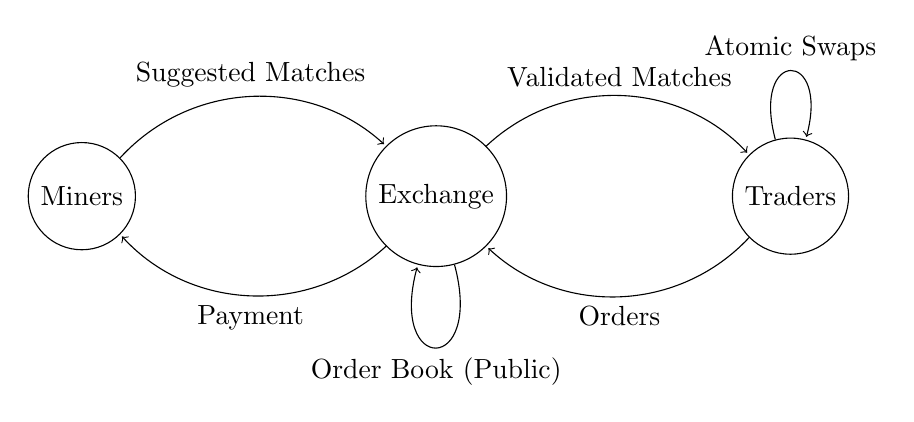
\begin{tikzpicture}[shorten >=1pt,node distance=4.5cm,
        					on grid]
  \node[state] (m)                {Miners};
  \node[state] (e) [right=of m] {Exchange};
  \node[state] (t) [right=of e] {Traders};
  \path[->] (m) edge [bend left=45] node [above] {Suggested Matches}
  																(e)
            (e) edge [loop below]   node  {Order Book (Public)} ()
            	edge [bend left=45] node [above] {Validated Matches}
            											(t)
            	edge [bend left=45]   node [below] {Payment} (m)
            (t) edge [loop above]   node {Atomic Swaps} ()
            	edge [bend left=45]   node [below] {Orders} (e);
		\end{tikzpicture}
        \end{center}
        \end{small}
\addcontentsline{toc}{section}{Order Matching}
\section*{Order Matching}
	Orders contain specifications on
    the currencies to be exchanged, volume, addresses of the trader,
    and price limit. They are sent with an Ether deposit, which is fully
    refunded on successful execution of the trade or partially refunded on
    withdrawal of the trade prior to execution. Orders are also sent with
    a predetermined amount of Ether to pay for gas and fees. The fees required are proportionate to the volume ordered. These orders
    are submitted by traders to the exchange, which then stores them in a
    public order book. Miners can access this information to make matches,
    which are then executed as trustless trades.

	The task of finding appropriate order matches is delegated to
    miners. These matches are then verified by the exchange.
	Matches are made such that the net exchange between currencies is
    within a specified margin as a percentage of the trade volume.
    The uncleared volume is reentered into the order book.
    Limits must also be non-contradictory. Matches found
    are rewarded according to the volume of currency exchanged in
    the transaction.
    To prevent attacks, miners will initially pay
    for any gas cost incurred in the network's verification of
    their proposal. This will be refunded on successful
    validation of the proposed match and instead paid for by the
    trading parties. Much like the factorization problem used in Bitcoin
    mining, the verification of a proposition is much less
    computationally demanding than the generation of a correct solution.
    This is because the matching problem used in the Valence protocol
    reduces to a subset-sum problem, which, like the factorization
    problem, is NP-complete.
\addcontentsline{toc}{section}{Token}
\section*{Token}
    A key component of an implementation of the Valence protocol is
    an ERC20-compliant token issued on the
    Ethereum platform. The initial supply of this token is
    implementation-specific.

		Each token grants its holder the right to a transferable vote on
    development decisions relevant to the platform.
	The inclusion of voting rights adds longevity to the system by
    allowing it to adapt to external changes. For example, a rise in
    popularity of a new cryptocurrency could be capitalized on by
    the addition to the exchange of transactions on that currency.
    Their transferability enables participation rates to remain
    sufficiently high by allowing miners who are less interested
    in the active development of the platform to transfer their
    voting rights to a more involved party. To prevent a majority coalition
    from abusing their amendment rights, all changes will be subject to a
    waiting period before being enacted.
		Token holders are also entitled to dividends, which come from the exchange's profits from collecting trading fees. Dividends are distributed at random intervals to reduce transactional costs and lower volatility.

\addcontentsline{toc}{section}{Examples}
\section*{Examples}
	\addcontentsline{toc}{subsection}
    	{Example 1: A Simple Transaction}
	\subsection*{Example 1: A Simple Transaction}
    	Alice wants to buy 14 Ether for at most 1 Bitcoin. Bob wants
        to buy 1 Bitcoin for at most 16 Ether. Mary the miner's job
        is to match orders.

        Alice submits her order, shown below, to the exchange:
        \begin{center}
        \scalebox{0.8}{
        \begin{tabular}{| c || c |}
        	\hline
            \texttt{Unit} & \texttt{ETH-BTC}  \\
            \hline
            \texttt{Quantity} & \texttt{14} \\
            \hline
            \texttt{Unit Limit} & \texttt{0.07} \\
            \hline
            \texttt{Buy Address} & \texttt{35 Unger Ln} \\
            \hline
            \texttt{Sell Address} & \texttt{12650 Corte Madera Ln} \\
            \hline
            \texttt{Order ID} & \texttt{ALICE} \\
            \hline
        \end{tabular}
        }
        \end{center}

        Bob also submits his order to the exchange:
        \begin{center}
        \scalebox{0.8}{
        \begin{tabular}{| c || c |}
        	\hline
            \texttt{Unit} & \texttt{BTC-ETH}  \\
            \hline
            \texttt{Quantity} & \texttt{1}  \\
            \hline
            \texttt{Unit Limit} & \texttt{16} \\
            \hline
            \texttt{Buy Address} & \texttt{1000 Corte Madera Ln} \\
            \hline
            \texttt{Sell Address} & \texttt{9 Unger Ln} \\
            \hline
            \texttt{Order ID} & \texttt{BOB} \\
            \hline
        \end{tabular}
        }
        \end{center}

        The exchange adds both orders to their order book, which
        already contains some orders:
        \begin{center}
        \scalebox{0.8}{
        \begin{tabular}{| c || c | c | c | c |}
        	\hline
            \texttt{Unit} & \texttt{BTC-ETH} & \texttt{ETH-BTC}
            		& \texttt{ETH-BTC} & \texttt{BTC-ETH}\\
            \hline
            \texttt{Quantity} & \texttt{2} & \texttt{33}
            		& \texttt{14} & \texttt{1}\\
            \hline
            \texttt{Unit Limit} & \texttt{16} & \texttt{0.07}
            		& \texttt{0.07} & \texttt{16} \\
            \hline
            \texttt{Buy Address} & \texttt{1500 Corte Madera Ln}
            		& \texttt{22 Unger Ln} & \texttt{35 Unger Ln}
                    & \texttt{1000 Corte Madera Ln} \\
            \hline
            \texttt{Sell Address} & \texttt{4 Unger Ln}
            		& \texttt{1345 Corte Madera Ln}
                    & \texttt{12650 Corte Madera Ln}
                    & \texttt{9 Unger Ln} \\
            \hline
            \texttt{Order ID} & \texttt{CAROL} & \texttt{DAVE}
            		& \texttt{ALICE} & \texttt{BOB} \\
            \hline
        \end{tabular}
        }
        \end{center}

        Mary sees that the order book has been updated and matches
        Alice and Bob's orders. She suggests this match to the
        exchange at a mutually acceptable exchange rate, 15 Ether
        per Bitcoin.
        The match is valid,
        so the exchange gives Mary
        a portion of the fees it receives from Alice and Bob. The exchange then creates an atomic swap contract
        for Alice and Bob, who
        trustlessly trade. Their entries in the order book are
        cleared.

	\addcontentsline{toc}{subsection}
        {Example 2: A Transaction with a Remainder}
	\subsection*{Example 2: A Transaction with a Remainder}
    	After Alice and Bob's transaction is cleared, only
        Carol and Dave's orders are still in the order book:
        \begin{center}
        \scalebox{0.8}{
        \begin{tabular}{| c || c | c |}
        	\hline
            \texttt{Unit} & \texttt{BTC-ETH} & \texttt{ETH-BTC} \\
            \hline
            \texttt{Quantity} & \texttt{2} & \texttt{33} \\
            \hline
            \texttt{Unit Limit} & \texttt{16} & \texttt{0.07} \\
            \hline
            \texttt{Buy Address} & \texttt{1500 Corte Madera Ln}
            		& \texttt{22 Unger Ln} \\
            \hline
            \texttt{Sell Address} & \texttt{4 Unger Ln}
            		& \texttt{1345 Corte Madera Ln}  \\
            \hline
            \texttt{Order ID} & \texttt{CAROL} & \texttt{DAVE} \\
            \hline
        \end{tabular}
        }
        \end{center}
        As before, Mary suggests a match between Carol and Dave's
        orders at an exchange rate of 15 Ether per Bitcoin. There's
        a slight problem, though: this exchange rate leaves Dave's
        order with three remaining Ether on the order book. On
        validation of the match, however, the exchange finds that as
        a percentage of the total trade this deficiency is
        within its implementation-specific margin for
        error. Then the exchange rewards Mary for finding the match,
        and creates a smart contract for Carol and Dave to
        trade. Carol's order is cleared, while the remainder
        of Dave's order is reentered into the order book. The order
        book, shown below, now only contains the remainder of Dave's
        order.

        \begin{center}
        \scalebox{0.8}{
        \begin{tabular}{| c || c | c |}
        	\hline
            \texttt{Unit} & \texttt{ETH-BTC} \\
            \hline
            \texttt{Quantity} & \texttt{3} \\
            \hline
            \texttt{Unit Limit} & \texttt{0.07} \\
            \hline
            \texttt{Buy Address} & \texttt{22 Unger Ln} \\
            \hline
            \texttt{Sell Address} & \texttt{1345 Corte Madera Ln}  \\
            \hline
            \texttt{Order ID} & \texttt{DAVE} \\
            \hline
        \end{tabular}
        }
        \end{center}
\addcontentsline{toc}{section}{Challenges and Resolutions}
\section*{Challenges and Resolutions}
  \addcontentsline{toc}{subsection}{Latency and Scalability}
  \subsection*{Latency and Scalability}
  	A significant challenge faced by exchanges is maintaining low latency
    as the system scales.
    The system outlined by the Valence protocol should prove to be
    highly scalable. Updating the order book is inexpensive,
    and the on-blockchain operational cost is constant.
    Because few operations are performed on the blockchain by the exchange,
    the latency of transacting will be competitive with that of a
    centralized exchange.

    To further increase efficiency at scale, we recommend the establishment
    of a convention whereby miners attempt to match trades of volumes
    proportionate to their computing power. This convention dramatically
    lowers the number of colliding suggested trades and decreases the
    latency with which orders are matched, increasing expected transactional
    value for both miners and traders. From a game-theoretical perspective,
    the strategy of adhering to the convention is evolutionarily stable, in
    that no party has an incentive to defect from the convention. Miners
    will not choose to match orders of lower value than their assigned
    bracket, because the yields will be lower. Similarly, they have no
    reason to match orders of a higher value than their assigned bracket,
    because they will be consistently be outpaced by competitors with more
    computing power.
  \addcontentsline{toc}{subsection}{Market Manipulation by Miners}
  \subsection*{Market Manipulation by Miners}
  	Public order books have been criticized for enabling miners to front-run
    existing orders by placing their own orders and matching
    them.\footnote[6]{\url{https://swap.tech/whitepaper/\#order-books}}
    Because orders are public, and not exclusively visible to miners, this
    analogy to classical front-running is fallacious.
    In reality, trading miners provide liquidity using only publicly
    available information, in a manner more akin to high-frequency
    traders on classical exchanges. Placing price limits on orders is always
    best practice, especially on an exchange with a public order book, but
    miners are in no way empowered to match orders that are not consensual
    for all parties involved.
  \addcontentsline{toc}{subsection}{Barriers to Entry}
  \subsection*{Barriers to Entry}
  	Atomic swaps do not support fiat currencies.
  	Because the Valence protocol depends on atomic swaps, it cannot
    facilitate transactions involving a fiat currency. While this is a
    significant entry barrier for parties not holding cryptocurrencies,
    fiat currency transactions inherently require trust, so this deficiency
    is inevitable in a trustless system.

    Additionally, because the exchange is implemented as an Ethereum smart
    contract, traders must possess a small amount of Ether to be able to pay
    transaction fees. This shortcoming is potentially problematic for
    smaller participants, but should not be an issue for more sophisticated
    traders, who tend to hold positions in both Ether and Bitcoin.
    To overcome this barrier, prospective traders with no Ether can
    perform a small transaction with a known broker, using information
    acquired from a Valence implementation's recent transactions for pricing
    data. They can then use the Ether acquired from this transaction to
    obtain a larger quantity using an implementation of Valence.

    Because of its design as a completely trustless system, the outlined
    protocol does not require traders or miners to register.
    %Unlike
    %competing approaches such as OmegaOne,\footnote[7]
    %{\url{https://omega.one/}}
    there is also no minimum token balance to trade.
    This removes a
    significant entry barrier faced by centralized exchanges.
  \addcontentsline{toc}{subsection}{Competition}
  \subsection*{Competition}
    An implementation of this protocol would also compete with other planned decentralized cryptocurrency exchanges such as KyberNetwork. Often, however, these exchanges primarily aim to support trading Ethereum tokens, with cross-blockchain transactions as an afterthought. In the case of KyberNetwork, for example, there is no plan to support cross-blockchain trading until 2019.\footnote[7]{\url{https://kyber.network/\#roadmap}} Additionally, KyberNetwork depends on a reserve-management model, which poses significant security risks and is potentially prone to exchange rate fixing by malevolent reserve managers.\footnote[8]
        {\url{https://kyber.network/assets/KyberNetworkWhitepaper.pdf}}

    Existing and planned token exchanges like AirSwap, Bancor, and 0x are orthogonal to Valence, and would not compete with a Valence implementation. Atomic swap contracts for exchanging tokens on the Ethereum blockchain are significantly different from those for cross-blockchain transactions, so for any of these exchanges to expand into competing with a Valence implementation would be a substantial undertaking.

    Dark pools such as OmegaOne serve an adjacent but separate role from Valence. Due to their high barriers to entry, they are largely inaccessible to even sophisticated traders without an agreement with a specialized broker. Furthermore, because OmegaOne is not a freestanding exchange, but rather splits up large orders it receives and distributes them among various exchanges, its relationship with Valence would actually be a mutualistic one, so the success of either would be beneficial to the other.

\addcontentsline{toc}{section}{Conclusion}
\section*{Conclusion}
	The Valence protocol outlines the creation of a
    decentralized
    cryptocurrency exchange using atomic swaps for trustless trades.
    this protocol has high value if
    faithfully implemented, and, utilizing technologies that are
    novel for an exchange, fixes the serious issue of
    counterparty risk in its domain.

\end{document}
